\documentclass[9pt]{extarticle}
\usepackage{fontspec}
\setmainfont{Leelawadee UI}
\usepackage[a4paper,top=0.7cm,bottom=0.7cm,left=0.7cm,right=0.7cm]{geometry}
\usepackage{multicol}
\setlength{\columnsep}{0.45cm}
\setlength{\columnseprule}{0.4pt}
\usepackage{amsmath,amssymb}
\usepackage{xcolor}
\usepackage{colortbl}
\usepackage{tikz}
\usepackage{pgfplots}
\pgfplotsset{compat=1.18}
\usepackage{enumitem}
\setlist{nosep,leftmargin=1.1em,itemsep=0pt,topsep=1pt}
\usepackage{titlesec}
\usepackage{tcolorbox}
\tcbuselibrary{skins}

\definecolor{navy}{RGB}{20,40,90}
\definecolor{gold}{RGB}{190,140,20}
\definecolor{lightbg}{RGB}{240,244,250}
\definecolor{solbg}{RGB}{247,247,240}
\definecolor{ideabg}{RGB}{236,246,238}
\definecolor{ideafr}{RGB}{60,120,70}

\titleformat{\section}{\normalfont\bfseries\normalsize\color{navy}}{\thesection}{0.4em}{}[{\color{gold}\titlerule[1pt]}]
\titlespacing*{\section}{0pt}{4pt}{2pt}
\titleformat{\subsection}{\normalfont\bfseries\color{gold}}{\thesubsection}{0.3em}{}
\titlespacing*{\subsection}{0pt}{2pt}{0pt}

\newtcolorbox{formulabox}{
  colback=lightbg, colframe=navy!60, boxrule=0.4pt,
  arc=1pt, left=3pt, right=3pt, top=1pt, bottom=1pt,
  fontupper=\footnotesize
}
\newtcolorbox{solbox}{
  colback=solbg, colframe=gold!70!black, boxrule=0.4pt,
  arc=1pt, left=3pt, right=3pt, top=1.5pt, bottom=1.5pt,
  fontupper=\footnotesize
}
\newtcolorbox{ideabox}{
  colback=ideabg, colframe=ideafr, boxrule=0.4pt,
  arc=1pt, left=3pt, right=3pt, top=1.5pt, bottom=1.5pt,
  fontupper=\footnotesize
}

\newcommand{\dist}[1]{\subsection*{\textcolor{navy}{\textbullet\ #1}}}
\newcommand{\howto}{\textbf{\textcolor{navy!70!black}{วิธีอ่านตาราง:}}\ }

\setlength{\parindent}{0pt}
\setlength{\parskip}{0.5pt}

\pgfplotsset{
  every axis/.append style={
    label style={font=\tiny}, tick label style={font=\tiny},
    width=4.0cm, height=2.3cm, axis lines=left,
    xlabel={$x$}, ylabel={$P(X{=}x)$},
    xlabel style={yshift=2pt}, ylabel style={yshift=-2pt},
    tick align=outside, ymin=0, enlarge x limits={abs=0.35},
    axis line style={-latex, thin}, ticklabel style={/pgf/number format/fixed}
  }
}
\setlength{\abovedisplayskip}{2pt}
\setlength{\belowdisplayskip}{2pt}
\setlength{\abovedisplayshortskip}{1pt}
\setlength{\belowdisplayshortskip}{1pt}

\pgfmathdeclarefunction{gauss}{3}{%
  \pgfmathparse{1/(#3*sqrt(2*pi))*exp(-((#1-#2)^2)/(2*#3^2))}%
}

\begin{document}
\begin{center}
{\Large\bfseries\color{navy} Chapter 2: ตัวแปรสุ่ม และการแจกแจงความน่าจะเป็น (Part 2)}\\[2pt]
{\small สรุปเนื้อหา — อ.ดร.ธนวรรณ ประฮาดไชย \quad Department of Statistics, Faculty of Science, KKU}
\end{center}
\vspace{2pt}
{\color{gold}\hrule height 1.4pt}
\vspace{4pt}

\begin{multicols}{3}

\section*{1. ตัวแปรสุ่มและค่าคาดหวัง}
\textbf{ตัวแปรสุ่ม (Random Variable)} คือ\allowbreak ตัวแปรที่มี\allowbreak ค่าเป็นตัวเลข\allowbreak ซึ่งได้จาก\allowbreak ผลลัพธ์ของ\allowbreak การทดลองสุ่ม แบ่งเป็น 2 ชนิด คือ ตัวแปรสุ่ม\textbf{ชนิดไม่ต่อเนื่อง} (discrete) และ\textbf{ชนิดต่อเนื่อง} (continuous)

\textbf{การแจกแจงความน่าจะเป็น} คือ การแสดง\allowbreak ค่าที่เป็นไปได้\allowbreak ทั้งหมดของ\allowbreak ตัวแปรสุ่ม คู่กับ\allowbreak ความน่าจะเป็น\allowbreak ของแต่ละค่า

\begin{formulabox}
ค่าคาดหวัง (Expected value):
$$\mu = E(X) = \sum_x x\,P(X{=}x)$$
ความแปรปรวน (Variance):
$$\sigma^2 = Var(X) = E(X^2)-[E(X)]^2$$
ส่วนเบี่ยงเบนมาตรฐาน (SD):
$$\sigma = \sqrt{Var(X)}$$
\end{formulabox}

\section*{2. การแจกแจงความน่าจะเป็น\\ชนิดไม่ต่อเนื่อง (Discrete)}

\dist{เอกรูป (Discrete Uniform)}
เกิดจากการทดลองสุ่มที่มีผลลัพธ์ตั้งแต่ 2 ค่าขึ้นไป โดยแต่ละค่ามีโอกาสเกิดขึ้น\textbf{เท่า ๆ กัน}
\begin{formulabox}
$$P(X{=}x)=\dfrac{1}{k},\quad x=x_1,x_2,\dots,x_k$$
$$\mu=\dfrac{\sum x_i}{k}, \qquad \sigma^2=\dfrac{\sum (x_i-\mu)^2}{k}$$
\end{formulabox}

\textit{ตัวอย่าง 1:} ทอดลูกเต๋าเที่ยงตรง 1 ลูก 1 ครั้ง ให้ $X$ แทนแต้มที่หงาย จงหาความน่าจะเป็นที่ลูกเต๋าจะหงายหน้าอย่างมาก 4 แต้ม
\begin{ideabox}
\textbf{แนวคิด:} ผลลัพธ์มีได้ 6 ค่า (1--6) และลูกเต๋า\allowbreak เที่ยงตรง แต่ละค่าจึงมีโอกาส\allowbreak เกิด\textbf{เท่ากัน} $\to$ ตรงนิยาม\allowbreak การแจกแจง\allowbreak เอกรูป
\end{ideabox}
\begin{solbox}
$X=1,\dots,6$, $n(S)=6$, $P(X{=}x)=\frac16$\\
ต้องการ $P(X\le4)=P(1){+}P(2){+}P(3){+}P(4)$\\
$=4\left(\frac16\right)=\frac{2}{3}\approx 0.6667$
\end{solbox}

\begin{center}
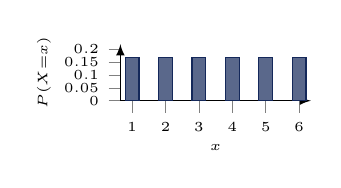
\begin{tikzpicture}
\begin{axis}[ybar, bar width=5pt, ymax=0.22, xtick={1,...,6}]
\addplot[fill=navy!70,draw=navy] coordinates {
(1,0.1667)(2,0.1667)(3,0.1667)(4,0.1667)(5,0.1667)(6,0.1667)};
\end{axis}
\end{tikzpicture}
\end{center}

\dist{แบร์นูลลี (Bernoulli)}
ได้จากการทดลองสุ่มที่มีผลลัพธ์เพียง 2 อย่าง คือ ความสำเร็จ (Success) และความไม่สำเร็จ (Failure)
\begin{formulabox}
$$P(X{=}x)=p^x q^{1-x},\quad x=0,1;\ q=1-p$$
$$\mu = p, \qquad \sigma^2 = pq$$
\end{formulabox}

\textit{ตัวอย่าง 2:} นักบาสเกตบอล\allowbreak ทีมชาติ\allowbreak โยนลงห่วง\allowbreak ได้ร้อยละ 75 จงหา\allowbreak ความน่าจะเป็น\allowbreak ที่เขาจะโยน\textbf{ไม่ลง}ห่วง
\begin{ideabox}
\textbf{แนวคิด:} โยน\allowbreak เพียง\textbf{ครั้งเดียว} ผลลัพธ์มี\allowbreak เพียง 2 อย่าง (ลง/ไม่ลง) $\to$ ตรงนิยาม\allowbreak แบร์นูลลี (ถ้าโยน\allowbreak หลายครั้ง\allowbreak อิสระกัน จะกลาย\allowbreak เป็นทวินาม)
\end{ideabox}
\begin{solbox}
$p=0.75$ (ลงห่วง), $q=1-0.75=0.25$ (ไม่ลงห่วง)\\
ต้องการ $P(X{=}0)=q=0.25$
\end{solbox}

\begin{center}
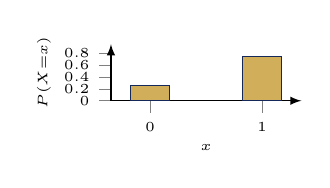
\begin{tikzpicture}
\begin{axis}[ybar, bar width=14pt, ymax=0.95, xtick={0,1}]
\addplot[fill=gold!70,draw=navy] coordinates {(0,0.25)(1,0.75)};
\end{axis}
\end{tikzpicture}
\end{center}

\dist{ทวินาม (Binomial)}
ทดลองสุ่ม $n$ ครั้งเหมือนกัน แต่ละครั้งเป็นอิสระต่อกัน มีผลลัพธ์ 2 อย่าง (สำเร็จ/ไม่สำเร็จ) และ $p$ คงที่ทุกครั้ง
\begin{formulabox}
$$P(X{=}x)=\binom{n}{x}p^x q^{n-x},\ x=0,1,\dots,n$$
$$\mu = np, \qquad \sigma^2 = npq$$
\end{formulabox}

\howto ตารางที่ I ให้ค่าสะสม $P(X\le x)=\sum_{k=0}^{x}P(X{=}k)$
\begin{enumerate}
\item เลือกตารางที่ตรงกับค่า $n$
\item หาแถวที่ตรงกับค่า $x$ (คอลัมน์ซ้ายสุด)
\item หาคอลัมน์ที่ตรงกับค่า $p$ (หัวตาราง)
\item ค่าตรงจุดตัดคือ $P(X\le x)$
\item $P(X{=}x)=P(X\le x)-P(X\le x{-}1)$
\item $P(X\ge x)=1-P(X\le x{-}1)$
\item $P(a\le X\le b)=P(X\le b)-P(X\le a{-}1)$
\end{enumerate}
หรือใช้ Excel: \texttt{BINOM.DIST}\allowbreak\texttt{(x,n,p,cum.)}

\textit{ตัวอย่าง 3:} ข้อสอบปรนัย 10 ข้อ แต่ละข้อมี 5 ตัวเลือก คำตอบถูก 1 ข้อ จงหา ก) $P$(ตอบถูกอย่างมาก 6 ข้อ) ข) ค่าเฉลี่ย\allowbreak และส่วนเบี่ยงเบน\allowbreak มาตรฐานของ\allowbreak จำนวนข้อที่ตอบถูก
\begin{ideabox}
\textbf{แนวคิด:} ทำซ้ำ 10 ครั้ง\allowbreak เหมือนกัน (10 ข้อ) แต่ละข้อ\allowbreak เป็นอิสระต่อกัน มีผล 2 อย่าง (ถูก/ผิด) และ $p$ คงที่\allowbreak ทุกข้อ $\to$ ครบ 4 เงื่อนไข\allowbreak ของทวินาม
\end{ideabox}
\begin{solbox}
$n=10,\ p=\frac15=0.2$\\
ก) ต้องการ $P(X\le6)$:\\ จากตาราง I แถว $x{=}6$\\ คอลัมน์ $p{=}0.20$\\
$P(X\le6)=0.9991$\\
ข) $\mu=np=10(0.2)=2$\\
$\sigma^2=npq=10(0.2)(0.8)=1.6$\\
$\sigma=\sqrt{1.6}\approx1.2649$
\end{solbox}

\begin{center}
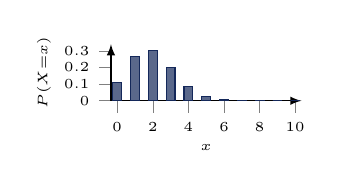
\begin{tikzpicture}
\begin{axis}[ybar, bar width=3.2pt, ymax=0.34, xtick={0,2,4,6,8,10}]
\addplot[fill=navy!70,draw=navy] coordinates {
(0,0.1074)(1,0.2684)(2,0.3020)(3,0.2013)(4,0.0881)
(5,0.0264)(6,0.0055)(7,0.0008)(8,0.0001)(9,0.0000)(10,0.0000)};
\end{axis}
\end{tikzpicture}
\end{center}

\dist{ไฮเพอร์จีออเมตริก (Hypergeometric)}
สิ่งของทั้งหมด $N$ สิ่ง แบ่งเป็นกลุ่มที่สนใจ $M$ สิ่ง และกลุ่มที่ไม่สนใจ $N{-}M$ สิ่ง สุ่มตัวอย่าง $n$ สิ่ง \textbf{แบบไม่ใส่คืน}
\begin{formulabox}
$$P(X{=}x)=\dfrac{\binom{M}{x}\binom{N-M}{n-x}}{\binom{N}{n}}$$
$$\mu = \dfrac{nM}{N}, \qquad \sigma^2 = n\dfrac{M}{N}\left(1-\dfrac{M}{N}\right)\dfrac{N-n}{N-1}$$
\end{formulabox}
Excel: \texttt{HYPGEOM.DIST(x,n,M,N,cum.)}

\textit{ตัวอย่าง 4:} พนักงานบริหาร 12 คน (หญิง 7, ชาย 5) สุ่มเลือก 3 คนพร้อมกัน จงหา ก) $P$(เป็นหญิงทั้ง 3 คน) ข) $P$(เป็นหญิงอย่างมาก 1 คน)
\begin{ideabox}
\textbf{แนวคิด:} สุ่มจาก\allowbreak ประชากรจำกัด (12 คน) แบบ\allowbreak \textbf{ไม่ใส่คืน} (เลือก\allowbreak พร้อมกันทีเดียว) แบ่งเป็น 2 กลุ่ม (หญิง/ชาย) $\to$ ต่างจาก\allowbreak ทวินามตรงที่\allowbreak สัดส่วนเปลี่ยน\allowbreak หลังเลือกแต่ละ\allowbreak คน จึงต้องใช้\allowbreak ไฮเพอร์จีออเมตริก
\end{ideabox}
\begin{solbox}
$N{=}12,\ M{=}7,\ n{=}3$\\
ก) $P(X{=}3)=\dfrac{\binom{7}{3}\binom{5}{0}}{\binom{12}{3}}=\dfrac{35(1)}{220}=0.1591$\\
ข) $P(X\le1)=P(0)+P(1)$\\
$=\dfrac{\binom{7}{0}\binom{5}{3}}{220}+\dfrac{\binom{7}{1}\binom{5}{2}}{220}$\\
$=0.0455+0.3182=0.3636$
\end{solbox}

\begin{center}
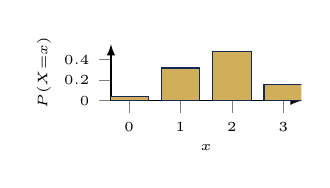
\begin{tikzpicture}
\begin{axis}[ybar, bar width=14pt, ymax=0.55, xtick={0,1,2,3}]
\addplot[fill=gold!70,draw=navy] coordinates {
(0,0.0455)(1,0.3182)(2,0.4773)(3,0.1591)};
\end{axis}
\end{tikzpicture}
\end{center}

\columnbreak
\dist{ปัวส์ซง (Poisson)}
จำนวนครั้งของ\allowbreak การเกิดเหตุการณ์\allowbreak ในช่วงเวลา/\allowbreak ขอบเขตหนึ่ง โดยเหตุการณ์\allowbreak เป็นอิสระกัน เกิดขึ้นได้\allowbreak ไม่จำกัดจำนวนครั้ง และในช่วงสั้น ๆ ความน่าจะเป็น\allowbreak ของการเกิด\allowbreak มีค่าน้อย
\begin{formulabox}
$$P(X{=}x)=\dfrac{e^{-\lambda}\lambda^x}{x!},\quad x=0,1,2,\dots$$
$$\mu = \lambda, \qquad \sigma^2 = \lambda$$
\end{formulabox}

\howto ตารางที่ II ให้ค่าสะสม $P(X\le x)$ เช่นเดียวกับตาราง I แต่ใช้ $\lambda$ แทน $p$ เป็นหัวคอลัมน์
\begin{enumerate}
\item หาคอลัมน์ที่ตรงกับค่า $\lambda$
\item หาแถวที่ตรงกับค่า $x$
\item ค่าตรงจุดตัดคือ $P(X\le x)$
\item ใช้กฎเดียวกับตาราง I ในการหา $P(X{=}x)$, $P(X\ge x)$, $P(a\le X\le b)$
\end{enumerate}
หรือใช้ Excel: \texttt{POISSON.DIST}\allowbreak\texttt{(x,$\lambda$,cum.)}

\textit{ตัวอย่าง 5:} ถนนในชนบทมีรถวิ่งผ่านเฉลี่ยชั่วโมงละ 24 คัน จงหา $P$(รถวิ่งผ่านอย่างมาก 30 คัน ใน 1 ชม.)
\begin{ideabox}
\textbf{แนวคิด:} นับ\textbf{จำนวนครั้ง}ที่\allowbreak เหตุการณ์เกิด (รถผ่าน) ในช่วงเวลา\allowbreak หนึ่ง (1 ชม.) โดยไม่มี $n$ ตายตัว\allowbreak แบบทวินาม และแต่ละ\allowbreak เหตุการณ์เป็น\allowbreak อิสระกัน $\to$ ตรงนิยาม\allowbreak ปัวส์ซง
\end{ideabox}
\begin{solbox}
$X{=}$จำนวนรถที่วิ่งผ่านใน 1 ชม., $\lambda=24$\\
ต้องการ $P(X\le30)$: จากตาราง II แถว $x{=}30$ คอลัมน์ $\lambda{=}24$\\
$P(X\le30)=0.9042$
\end{solbox}

\textit{ตัวอย่าง 6 (ทวินาม$\to$ปัวส์ซง):} ความน่าจะเป็น\allowbreak ที่คนแต่ละคน\allowbreak ตาบอดสี $=0.001$ สุ่มคน 1{,}000 คน จงหา $P$(ตาบอดสีอย่างมาก 5 คน)
\begin{ideabox}
\textbf{แนวคิด:} จริง ๆ เป็น\allowbreak ทวินาม ($n{=}1000,p{=}0.001$) แต่ $n$ มาก\allowbreak มาก และ $p$ น้อยมาก\allowbreak (เหตุการณ์หายาก) การคำนวณ\allowbreak $\binom{1000}{x}$ ยุ่งยาก\allowbreak เกินไป จึง\textbf{ประมาณด้วย\allowbreak ปัวส์ซง}แทน ($\lambda{=}np$) เพื่อคำนวณ\allowbreak ง่ายขึ้น
\end{ideabox}
\begin{solbox}
$n{=}1000$ มาก, $p{=}0.001$ น้อย $\Rightarrow$ ประมาณด้วยปัวส์ซง\\
$\lambda=np=1000(0.001)=1$\\
ต้องการ $P(X\le5)$: จากตาราง II ที่ $\lambda{=}1.00$\\
$P(X\le5)=0.9994$
\end{solbox}

กราฟด้านล่าง\allowbreak แสดงรูปทรง\allowbreak ทั่วไปของ\allowbreak การแจกแจง\allowbreak ปัวส์ซง ($\lambda=6$)

\begin{center}
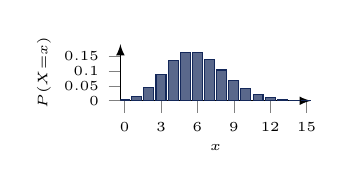
\begin{tikzpicture}
\begin{axis}[ybar, bar width=3.6pt, ymax=0.19, xtick={0,3,6,9,12,15}]
\addplot[fill=navy!70,draw=navy] coordinates {
(0,0.0025)(1,0.0149)(2,0.0446)(3,0.0892)(4,0.1339)(5,0.1606)
(6,0.1606)(7,0.1377)(8,0.1033)(9,0.0688)(10,0.0413)(11,0.0225)
(12,0.0113)(13,0.0052)(14,0.0022)(15,0.0009)};
\end{axis}
\end{tikzpicture}
\end{center}

\section*{3. การแจกแจงความน่าจะเป็น\\ชนิดต่อเนื่อง (Continuous)}

\dist{ปกติ (Normal Distribution)}
ใช้กับข้อมูลมาตรวัดอันตรภาค (interval) และอัตราส่วน (ratio) เช่น ส่วนสูง น้ำหนัก คะแนนสอบ รายได้ เส้นโค้งรูประฆังคว่ำ สมมาตรรอบค่าเฉลี่ย พื้นที่ใต้โค้งทั้งหมด $=1$
\begin{formulabox}
$$f(x)=\dfrac{1}{\sigma\sqrt{2\pi}}\,e^{-\frac{(x-\mu)^2}{2\sigma^2}},\ -\infty<x<\infty$$
พารามิเตอร์: $\mu$ (ค่าเฉลี่ย), $\sigma^2$ (ความแปรปรวน)
\end{formulabox}

\textit{ตัวอย่าง:} น้ำหนักมะเขือเทศ 300 ผล แจกแจงปกติ $\mu=68$ กรัม, $\sigma=3$ กรัม จงหา ก) ร้อยละของมะเขือเทศที่มีน้ำหนัก 64--72 กรัม ข) จำนวนผลที่คาดว่าจะมีน้ำหนักช่วงนี้
\begin{ideabox}
\textbf{แนวคิด:} น้ำหนักเป็น\allowbreak ข้อมูล\textbf{ต่อเนื่อง} (วัดค่าได้\allowbreak ละเอียด ไม่ใช่การนับ\allowbreak จำนวนครั้ง) และโจทย์\allowbreak ระบุว่า\allowbreak ``มีการแจกแจง\allowbreak ปกติ'' อยู่แล้ว $\to$ ใช้การแจกแจง\allowbreak ปกติ แปลงเป็น $Z$ เพื่อเปิด\allowbreak ตาราง III
\end{ideabox}
\begin{solbox}
$Z=\dfrac{X-\mu}{\sigma}$: $Z_1=\dfrac{64-68}{3}=-1.33$, $Z_2=\dfrac{72-68}{3}=1.33$\\
$P(64{<}X{<}72)=P(-1.33{<}Z{<}1.33)$\\
$=P(Z{<}1.33)-P(Z{<}-1.33)$\\
$=0.9082-0.0918=0.8164 \Rightarrow 81.64\%$\\
ข) $300\times0.8164\approx245$ ผล
\end{solbox}

\begin{center}
\vspace{-2pt}
\begin{tikzpicture}
\begin{axis}[width=4.6cm,height=2.4cm,axis lines=left,
  xlabel={$x$},ylabel={$f(x)$},ymin=0,ymax=0.15,
  xtick={59,62,65,68,71,74,77},tick label style={font=\tiny},
  label style={font=\tiny},axis line style={-latex,thin}]
\addplot[domain=59:77,samples=80,navy,thick] {gauss(x,68,3)};
\addplot[domain=64:72,samples=60,fill=gold!55,draw=none] {gauss(x,68,3)} \closedcycle;
\end{axis}
\end{tikzpicture}
\vspace{-4pt}
\end{center}

\dist{ปกติมาตรฐาน (Standard Normal)}
ถ้า $Z$ มีการแจกแจงแบบปกติที่ $\mu_Z=0,\ \sigma_Z^2=1$ เรียกว่าการแจกแจงแบบปกติมาตรฐาน
\begin{formulabox}
$$Z=\dfrac{X-\mu}{\sigma}$$
$$f(z)=\dfrac{1}{\sqrt{2\pi}}\,e^{-z^2/2}$$
\end{formulabox}

\howto ตารางที่ III ให้พื้นที่ใต้โค้งทางซ้ายของ $z$ คือ $P(Z<z)$
\begin{enumerate}
\item แยกค่า $z$ เป็นตำแหน่งจุดทศนิยมที่ 1 (แถว) กับตำแหน่งที่ 2 (คอลัมน์) เช่น $z{=}1.96$ $\to$ แถว 1.9 คอลัมน์ 0.06
\item ตารางแยกฝั่ง $z$ ลบ (ค่าน้อยกว่า 0) และฝั่ง $z$ บวก
\item ค่าตรงจุดตัดแถว--คอลัมน์ คือ $P(Z{<}z)$
\item ถ้าทราบพื้นที่\allowbreak (ความน่าจะเป็น) และต้องการ\allowbreak หา $z$ ให้ทำย้อนกลับ: ค้นหา\allowbreak ตัวเลขในตาราง\allowbreak ที่ใกล้เคียง\allowbreak พื้นที่ที่กำหนด แล้วอ่าน\allowbreak แถว/คอลัมน์นั้น\allowbreak ย้อนกลับเป็นค่า $z$
\end{enumerate}
สูตรที่ใช้บ่อย: $P(Z{>}z)=1-P(Z{<}z)$, $P(a{<}Z{<}b)=P(Z{<}b)-P(Z{<}a)$

\textit{ตัวอย่าง (อ่านตารางแบบตรง):} จงหา $P(0<Z<1.96)$
\begin{solbox}
$P(0{<}Z{<}1.96)=P(Z{<}1.96)-P(Z{<}0)$\\
$=0.975-0.5=0.475$
\end{solbox}

\textit{ตัวอย่าง (อ่านตารางแบบย้อนกลับ):} ถ้าทราบว่า $P(Z<z)=0.7734$ จงหาค่า $z$
\begin{solbox}
ค้นหา 0.7734 ในตาราง III $\to$ อยู่แถว 0.7 คอลัมน์ 0.05\\
ดังนั้น $z=0.75$
\end{solbox}
อีกตัวอย่าง: ถ้า $P(Z<z)=0.9850 \Rightarrow z=2.17$ (แถว 2.1 คอลัมน์ 0.07)

\begin{center}
\vspace{-2pt}
\begin{tikzpicture}
\begin{axis}[width=4.6cm,height=2.4cm,axis lines=left,
  xlabel={$z$},ylabel={$f(z)$},ymin=0,ymax=0.45,
  xtick={-3,-2,-1,0,1.96,3},tick label style={font=\tiny},
  label style={font=\tiny},axis line style={-latex,thin}]
\addplot[domain=-3.2:3.2,samples=80,navy,thick] {gauss(x,0,1)};
\addplot[domain=0:1.96,samples=40,fill=gold!55,draw=none] {gauss(x,0,1)} \closedcycle;
\end{axis}
\end{tikzpicture}
\vspace{-4pt}
\end{center}

\dist{การประมาณค่าด้วยโค้งปกติ}
เนื่องจากเป็น\allowbreak การประมาณ\allowbreak การแจกแจง\allowbreak ชนิดไม่ต่อเนื่อง\allowbreak ด้วยการแจกแจง\allowbreak ชนิดต่อเนื่อง จึงต้องปรับค่า $X$ ด้วย\allowbreak การบวก/ลบ $0.5$ เรียกว่า \textbf{``การปรับเพื่อให้ต่อเนื่อง'' (Correction for continuity)}

\begin{formulabox}
ทวินาม $\to$ ปกติ (เมื่อ $n$ มาก):
$$X\sim N(\mu,\sigma^2),\ \mu=np,\ \sigma^2=npq$$
ปัวส์ซง $\to$ ปกติ (เมื่อ $\lambda$ มาก):
$$X\sim N(\mu,\sigma^2),\ \mu=\lambda,\ \sigma^2=\lambda$$
\end{formulabox}

\textit{ตัวอย่าง:} รายงานวิจัยพบว่าร้อยละ 60 ของคนไทยสายตาสั้น สุ่มตัวอย่าง 100 คน จงหา ก) $P$(คนไทย 50 คนสายตาสั้น) ข) $P$(คนไทยมากกว่า 70 คนสายตาสั้น)
\begin{ideabox}
\textbf{แนวคิด:} จริง ๆ เป็น\allowbreak ทวินาม ($n{=}100,p{=}0.6$) แต่ $n$ มากพอ\allowbreak ($np{=}60\ge5$ และ $nq{=}40\ge5$) การคำนวณ\allowbreak $\binom{100}{x}$ ยุ่งยาก จึง\textbf{ประมาณด้วย\allowbreak โค้งปกติ}แทน และต้อง\allowbreak ปรับต่อเนื่อง ($\pm0.5$) เพราะใช้\allowbreak โค้งต่อเนื่องแทน\allowbreak ค่าที่นับเป็น\allowbreak จำนวนเต็ม
\end{ideabox}
\begin{solbox}
$\mu=np=100(0.6)=60$\\
$\sigma^2=npq=100(0.6)(0.4)=24,\ \sigma=\sqrt{24}\approx4.899$\\
ก) $P(X{=}50)\approx P(49.5{<}X{<}50.5)$\\
$Z_1=\frac{49.5-60}{4.899}=-2.14,\ Z_2=\frac{50.5-60}{4.899}=-1.94$\\
$=P(Z{<}{-1.94})-P(Z{<}{-2.14})$\\
$=0.0262-0.0162=0.0100$\\
ข) $P(X{>}70)\approx P(X{>}70.5)$\\
$Z=\frac{70.5-60}{4.899}=2.14$\\
$P(Z{>}2.14)=1-0.9838=0.0162$
\end{solbox}

\textit{ตัวอย่าง:} ตู้ ATM มีลูกค้าเฉลี่ย 35 คนต่อชั่วโมง ปิดซ่อม 1 ชั่วโมง จงหา ก) $P$(ลูกค้ามาใช้บริการ 40--50 คน) ข) $P$(ลูกค้ามาใช้บริการน้อยกว่า 40 คน)
\begin{ideabox}
\textbf{แนวคิด:} จริง ๆ เป็น\allowbreak ปัวส์ซง (นับจำนวน\allowbreak ลูกค้าในช่วงเวลา, $\lambda{=}35$) แต่ $\lambda$ มากพอ\allowbreak จึง\textbf{ประมาณด้วย\allowbreak โค้งปกติ}แทนเพื่อ\allowbreak คำนวณง่ายขึ้น ต้องปรับ\allowbreak ต่อเนื่องเช่นกัน
\end{ideabox}
\begin{solbox}
$\mu=\lambda=35,\ \sigma^2=\lambda=35,\ \sigma=\sqrt{35}\approx5.916$\\
ก) $P(40{\le}X{\le}50)\approx P(39.5{<}X{<}50.5)$\\
$Z_1=\frac{39.5-35}{5.916}=0.76,\ Z_2=\frac{50.5-35}{5.916}=2.62$\\
$=P(Z{<}2.62)-P(Z{<}0.76)=0.9956-0.7764=0.2192$\\
ข) $P(X{<}40)\approx P(X{<}39.5)$\\
$Z=\frac{39.5-35}{5.916}=0.76$\\
$P(Z{<}0.76)=0.7764$
\end{solbox}

\dist{ทวินาม $\to$ ปัวส์ซง}
เมื่อ $n\to\infty$, $p\to0$ และ $np=\lambda$ คงที่:
\begin{formulabox}
$$b(x;n,p)\ \approx\ f(x;\lambda),\quad \lambda=np$$
\end{formulabox}
(ดูตัวอย่าง 6 ในหัวข้อปัวส์ซงด้านซ้าย)

\section*{4. ตารางอ้างอิงฟังก์ชัน Excel}
\begin{formulabox}
\begin{tabular}{@{}ll@{}}
\textbf{ทวินาม} & \texttt{BINOM.DIST}\\
& \texttt{(x,n,p,cum.)}\\
\textbf{ไฮเพอร์จีออเมตริก} & \texttt{HYPGEOM.DIST}\\
& \texttt{(x,n,M,N,cum.)}\\
\textbf{ปัวส์ซง} & \texttt{POISSON.DIST}\\
& \texttt{(x,$\lambda$,cum.)}\\
\end{tabular}
\end{formulabox}

\textbf{ตารางความน่าจะเป็น:} ตาราง I = ทวินาม, ตาราง II = ปัวส์ซง, ตาราง III = ปกติมาตรฐาน — ทั้งสามตารางให้ค่าความน่าจะเป็น\textbf{สะสม} (cumulative) และอ่านด้วยวิธีตัดแถว--คอลัมน์แบบเดียวกัน

\textit{หมายเหตุ:} เอกรูป,\allowbreak แบร์นูลลี,\allowbreak ไฮเพอร์จีออเมตริก \textbf{ไม่มีเลขตาราง} เพราะเอกรูป/\allowbreak แบร์นูลลี\allowbreak คำนวณตรงจาก\allowbreak สูตรง่าย ๆ ได้เลย\allowbreak ส่วนไฮเพอร์จีออเมตริก\allowbreak มีพารามิเตอร์ 3 ตัว ($N,M,n$) จึงพิมพ์เป็น\allowbreak ตารางตายตัว\allowbreak ครอบคลุมไม่ได้ ต้องใช้สูตร\allowbreak หรือ Excel แทน

\end{multicols}
\newpage
\section*{5. ภาคผนวก: ค่าจริงจากตาราง}

\subsection*{\textcolor{ideafr}{ตารางนับสะสมจากฝั่งไหน?}}
\begin{center}
\begin{tabular}{cc}
\begin{minipage}{7.2cm}
\centering
\textbf{ตาราง I \& II (ไม่ต่อเนื่อง):} นับสะสมจาก $x=0$ \textbf{(ซ้ายสุด)} ไล่ไปทางขวาจนถึง $x$ ที่ต้องการ — แท่งทึบคือค่าที่รวมอยู่ใน $P(X\le x)$
\begin{tikzpicture}
\begin{axis}[ybar, bar width=13pt, ymax=0.28, xtick={0,...,8},
  width=7cm,height=3.6cm,
  label style={font=\small}, tick label style={font=\small},
  xlabel={$x$}, ylabel={$P(X{=}x)$}]
\addplot[fill=navy!70,draw=navy] coordinates {
(0,0.05)(1,0.11)(2,0.18)(3,0.22)(4,0.19)(5,0.13)};
\addplot[fill=white,draw=navy!50,dashed] coordinates {
(6,0.07)(7,0.03)(8,0.01)};
\draw[-latex,thick,gold] (axis cs:0,-0.045) -- (axis cs:5,-0.045)
  node[midway,below,font=\small,black]{นับจากซ้าย $\to$ ขวา};
\end{axis}
\end{tikzpicture}\\
{\footnotesize แท่งทึบ ($x{=}0$--$5$) $=P(X\le5)$; แท่งโปร่ง ($x{=}6$--$8$) ไม่ถูกนับรวม\par}
\end{minipage}
&
\begin{minipage}{7.2cm}
\centering
\textbf{ตาราง III (ต่อเนื่อง):} นับพื้นที่ใต้โค้งจาก $-\infty$ \textbf{(ซ้ายสุดของกราฟ)} ไล่มาทางขวาจนถึง $z$ ที่ต้องการ — พื้นที่แรเงาคือ $P(Z<z)$
\begin{tikzpicture}
\begin{axis}[width=7cm,height=3.6cm,axis lines=left,
  xlabel={$z$},ylabel={$f(z)$},ymin=0,ymax=0.45,
  xtick={-3,-2,-1,0,1,2,3},tick label style={font=\small},
  label style={font=\small},axis line style={-latex,thin}]
\addplot[domain=-3.4:3.4,samples=80,navy,thick] {gauss(x,0,1)};
\addplot[domain=-3.4:1,samples=60,fill=gold!55,draw=none] {gauss(x,0,1)} \closedcycle;
\draw[-latex,thick,gold!70!black] (axis cs:-3.2,-0.08) -- (axis cs:1,-0.08)
  node[midway,below,font=\small,black]{นับจากซ้าย $\to$ ขวา};
\end{axis}
\end{tikzpicture}\\
{\footnotesize พื้นที่แรเงา ($-\infty$ ถึง $z{=}1$) $=P(Z<1)$; ฝั่งขวาของ $z$ \textbf{ไม่ถูกนับ} (ถ้าต้องการต้องใช้ $1-P(Z<z)$)\par}
\end{minipage}
\end{tabular}
\end{center}

\begin{center}
\begin{tabular}{cc}
\begin{minipage}{7.5cm}
\centering
\subsection*{\textcolor{navy}{ตาราง I: ทวินามสะสม $P(X\le x)$ ($n{=}10$)}}
\small
\begin{tabular}{r|cccccc}
\rowcolor{lightbg} $x\backslash p$ & .10 & .20 & .25 & .30 & .40 & .50\\\hline
0 & .3487 & .1074 & .0563 & .0282 & .0060 & .0010\\
1 & .7361 & .3758 & .2440 & .1493 & .0464 & .0107\\
2 & .9298 & .6778 & .5256 & .3828 & .1673 & .0547\\
3 & .9872 & .8791 & .7759 & .6496 & .3823 & .1719\\
4 & .9984 & .9672 & .9219 & .8497 & .6331 & .3770\\
5 & .9999 & .9936 & .9803 & .9527 & .8338 & .6230\\
\textbf{6} & 1.000 & \textbf{.9991} & .9965 & .9894 & .9452 & .8281\\
7 & 1.000 & .9999 & .9996 & .9984 & .9877 & .9453\\
8 & 1.000 & 1.000 & 1.000 & .9999 & .9983 & .9893\\
9 & 1.000 & 1.000 & 1.000 & 1.000 & .9999 & .9990\\
\end{tabular}\\[3pt]
\small เช่น ตัวอย่าง 3: $x{=}6,p{=}.20 \Rightarrow P(X\le6){=}.9991$
\end{minipage}
&
\begin{minipage}{7.5cm}
\centering
\subsection*{\textcolor{navy}{ตาราง II: ปัวส์ซงสะสม $P(X\le x)$}}
\small
\begin{tabular}{r|ccccc}
\rowcolor{lightbg} $x\backslash \lambda$ & .90 & .95 & 1.00 & 1.10 & 1.20\\\hline
0 & .4066 & .3867 & .3679 & .3329 & .3012\\
1 & .7725 & .7541 & .7358 & .6990 & .6626\\
2 & .9371 & .9287 & .9197 & .9004 & .8795\\
3 & .9865 & .9839 & .9810 & .9743 & .9662\\
4 & .9977 & .9971 & .9963 & .9946 & .9923\\
\textbf{5} & .9997 & .9995 & \textbf{.9994} & .9990 & .9985\\
\end{tabular}\\[3pt]
\small เช่น ตัวอย่าง 6: $x{=}5,\lambda{=}1.00 \Rightarrow P(X\le5){=}.9994$\\[6pt]
\small\textit{หมายเหตุ:} $\lambda{=}24$ (ตัวอย่าง 5) เกินช่วงตารางมาตรฐานที่พิมพ์ในหนังสือ (ซึ่งมักมีถึงราว $\lambda{\approx}2$) จึงคำนวณด้วย Excel/ซอฟต์แวร์แทน — ค่ารอบ $x{=}30$ ที่คำนวณได้คือ:\\[3pt]
\begin{tabular}{r|ccc}
\rowcolor{lightbg} $x$ & 29 & \textbf{30} & 31\\\hline
$P(X\le x)$ & .8679 & \textbf{.9042} & .9322\\
\end{tabular}
\end{minipage}
\end{tabular}
\end{center}

\subsection*{\textcolor{navy}{ตาราง III: ปกติมาตรฐาน $P(Z<z)$ (ด้าน $z\ge0$; ด้าน $z<0$ ใช้สมมาตร $P(Z{<}{-z})=1-P(Z{<}z)$)}}
\begin{center}
{\scriptsize
\begin{tabular}{r|cccccccccc}
\rowcolor{lightbg} $z$ & .00 & .01 & .02 & .03 & .04 & .05 & .06 & .07 & .08 & .09\\\hline
0.0 & .5000 & .5040 & .5080 & .5120 & .5160 & .5199 & .5239 & .5279 & .5319 & .5359\\
0.1 & .5398 & .5438 & .5478 & .5517 & .5557 & .5596 & .5636 & .5675 & .5714 & .5753\\
0.2 & .5793 & .5832 & .5871 & .5910 & .5948 & .5987 & .6026 & .6064 & .6103 & .6141\\
0.3 & .6179 & .6217 & .6255 & .6293 & .6331 & .6368 & .6406 & .6443 & .6480 & .6517\\
0.4 & .6554 & .6591 & .6628 & .6664 & .6700 & .6736 & .6772 & .6808 & .6844 & .6879\\
0.5 & .6915 & .6950 & .6985 & .7019 & .7054 & .7088 & .7123 & .7157 & .7190 & .7224\\
0.6 & .7257 & .7291 & .7324 & .7357 & .7389 & .7422 & .7454 & .7486 & .7517 & .7549\\
0.7 & .7580 & .7611 & .7642 & .7673 & .7704 & \textbf{.7734} & \textbf{.7764} & .7794 & .7823 & .7852\\
0.8 & .7881 & .7910 & .7939 & .7967 & .7995 & .8023 & .8051 & .8078 & .8106 & .8133\\
0.9 & .8159 & .8186 & .8212 & .8238 & .8264 & .8289 & .8315 & .8340 & .8365 & .8389\\
1.0 & .8413 & .8438 & .8461 & .8485 & .8508 & .8531 & .8554 & .8577 & .8599 & .8621\\
1.1 & .8643 & .8665 & .8686 & .8708 & .8729 & .8749 & .8770 & .8790 & .8810 & .8830\\
1.2 & .8849 & .8869 & .8888 & .8907 & .8925 & .8944 & .8962 & .8980 & .8997 & .9015\\
1.3 & .9032 & .9049 & .9066 & \textbf{.9082} & .9099 & .9115 & .9131 & .9147 & .9162 & .9177\\
1.4 & .9192 & .9207 & .9222 & .9236 & .9251 & .9265 & .9279 & .9292 & .9306 & .9319\\
1.5 & .9332 & .9345 & .9357 & .9370 & .9382 & .9394 & .9406 & .9418 & .9429 & .9441\\
1.6 & .9452 & .9463 & .9474 & .9484 & .9495 & .9505 & .9515 & .9525 & .9535 & .9545\\
1.7 & .9554 & .9564 & .9573 & .9582 & .9591 & .9599 & .9608 & .9616 & .9625 & .9633\\
1.8 & .9641 & .9649 & .9656 & .9664 & .9671 & .9678 & .9686 & .9693 & .9699 & .9706\\
1.9 & .9713 & .9719 & .9726 & .9732 & .9738 & \textbf{.9744} & .9750 & .9756 & .9761 & .9767\\
2.0 & .9772 & .9778 & .9783 & .9788 & .9793 & .9798 & .9803 & .9808 & .9812 & .9817\\
2.1 & .9821 & .9826 & .9830 & .9834 & \textbf{.9838} & .9842 & .9846 & \textbf{.9850} & .9854 & .9857\\
2.2 & .9861 & .9864 & .9868 & .9871 & .9875 & .9878 & .9881 & .9884 & .9887 & .9890\\
2.3 & .9893 & .9896 & .9898 & .9901 & .9904 & .9906 & .9909 & .9911 & .9913 & .9916\\
2.4 & .9918 & .9920 & .9922 & .9925 & .9927 & .9929 & .9931 & .9932 & .9934 & .9936\\
2.5 & .9938 & .9940 & .9941 & .9943 & .9945 & .9946 & .9948 & .9949 & .9951 & .9952\\
2.6 & .9953 & .9955 & \textbf{.9956} & .9957 & .9959 & .9960 & .9961 & .9962 & .9963 & .9964\\
2.7 & .9965 & .9966 & .9967 & .9968 & .9969 & .9970 & .9971 & .9972 & .9973 & .9974\\
2.8 & .9974 & .9975 & .9976 & .9977 & .9977 & .9978 & .9979 & .9979 & .9980 & .9981\\
2.9 & .9981 & .9982 & .9982 & .9983 & .9984 & .9984 & .9985 & .9985 & .9986 & .9986\\
3.0 & .9987 & .9987 & .9987 & .9988 & .9988 & .9989 & .9989 & .9989 & .9990 & .9990\\
\end{tabular}
\par}
\end{center}
{\small ตัวเลขที่ \textbf{ตัวหนา} คือค่าที่ใช้ในตัวอย่างต่าง ๆ ของเอกสารนี้ (เช่น $z{=}0.75\to.7734$, $z{=}1.33\to.9082$, $z{=}1.96\to.9750$, $z{=}2.14\to.9838$, $z{=}2.17\to.9850$, $z{=}2.62\to.9956$)}

\end{document}
